\documentclass{report}
    \title{\vspace{-50pt}\textbf{\underline{COP4620 Notes}}}
    \author{William L. Thomson Jr.}
    \date{Spring Semester 2022}
    \addtolength{\textheight}{3cm}
    \usepackage{amsmath}
    \usepackage[T1]{fontenc}
    \usepackage[tmargin=1in,lmargin=1in,rmargin=1in]{geometry}
	\usepackage{titlesec}
    \usepackage{makecell}
    \usepackage{multicol}
    \usepackage{soul}
	\usepackage{enumitem}
    \usepackage{makecell}
	\usepackage{tikz}
	\usepackage{hyperref}
    \renewcommand\theadfont{\bfseries\sffamily}
    \usetikzlibrary{automata, positioning, arrows, babel,positioning,shapes}
    \tikzset{
        ->, % makes the edges directed
        >=stealth', % makes the arrow heads bold
        node distance=3cm, % minimum distance between two nodes. Change if necessary.
        every state/.style={thick, fill=gray!10}, % sets properties for each state node
        initial text=$ $, % sets the text that appears on the start arrow
    }
    \tikzstyle{vertex}=[draw,fill=black!15,circle,minimum size=20pt,inner sep=0pt]
    
	\hypersetup{ colorlinks=true, linkcolor=blue, filecolor=purple,urlcolor=cyan }
    
	\titleformat{\chapter}[display]
	{\bfseries\Large\itshape}
	{Chapter\ \thechapter}{0.5ex}{ }

	\titleformat{\section}
	{\normalfont\bfseries}
	{\thesection}{0.5em}{}

	\titleformat{\subsection}
	{\normalfont\bfseries}
	{\thesubsection}{0.5em}{}

    \titlespacing\chapter{0pt}{12pt plus 0pt minus 4pt}{0pt plus 0pt minus 4pt}
    \titlespacing\section{0pt}{12pt plus 4pt minus 8pt}{0pt plus 2pt minus 8pt}
    \titlespacing\subsection{0pt}{12pt plus 4pt minus 4pt}{0pt plus 2pt minus 4pt}
    \titlespacing\subsubsection{0pt}{12pt plus 4pt minus 2pt}{0pt plus 2pt minus 2pt}

    \setlist[description]{noitemsep, topsep=0pt, itemsep=-.1em}
    \setlist[enumerate]{noitemsep, topsep=0pt, itemsep=-.1em}
    \setlist[itemize]{noitemsep, topsep=0pt, itemsep=-.1em}
    \setlist[trivlist]{noitemsep, topsep=-8pt, itemsep=-.1em}

    \newcommand{\comment}[1]{}

\begin{document}

\maketitle
\tableofcontents


\renewcommand\thechapter{Q1}
\chapter{Take Home Quiz 1}
\section{Question 2}
\noindent The RE for the following: "All strings of x's and y's ending with xx or xy" \textbf{(x|y)*x(x|y)}

\section{Question 3}
\noindent RE: a(bab)*|a(ba)*\newline
  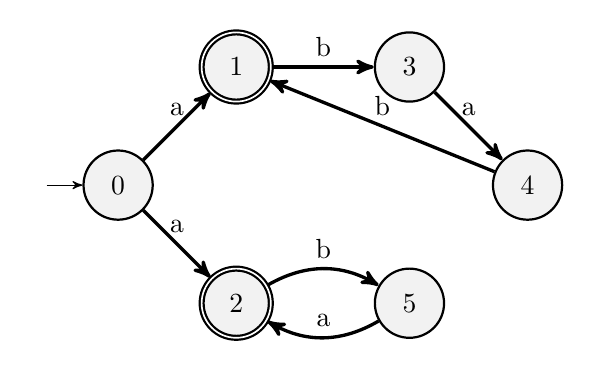
\begin{tikzpicture}[node distance=1.5cm]
    \node[state, initial] (0) {$0$};
    \node[state, accepting, above of=0, right of=0] (1) {$1$};
    \node[state, accepting, below of=0, right of=0] (2) {$2$};
    \node[state, right of=1, xshift=7mm] (3) {$3$};
    \node[state, below of=3, right of=3] (4) {$4$};
    \node[state, right of=2, xshift=7mm] (5) {$5$};
    \draw[very thick]
      (0) edge[left, above] node{a} (1)
      (0) edge[left, above] node{a} (2)
      (1) edge[left, above] node{b} (3)
      (2) edge[bend left, above] node{b} (5)
      (3) edge[left, above] node{a} (4)
      (4) edge[left, above] node{b} (1)
      (5) edge[bend left, above] node{a} (2);
  \end{tikzpicture}

\section{Question 4}
\noindent Consider the given NFA and its corresponding DFA (transition table) generated by applying the subset construction algorithm discussed in the class.
\vspace{-1em}
\begin{multicols}{2}
  \begin{tabular}{|c|c|c|c|c|}
    \hline
	 \thead{Index} & \thead{State} & \thead{a} & \thead{b} & \thead{Final?} \\
    \hline
	\textbf{1} & \{0\}   & \{1,2\} & err     & Yes \\
    \hline
	\textbf{2} & \{1,2\} & \{1,2\} & \{1,3\} & Yes \\
    \hline
	\textbf{3} & \{1,3\} & \{1,2\} & err     & Yes \\
    \hline
  \end{tabular}\newline\newline
  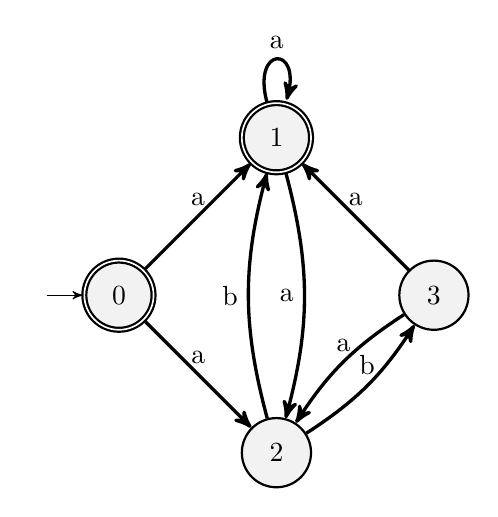
\begin{tikzpicture}[node distance=2cm]
    \node[state, accepting, initial] (0) {$0$};
    \node[state, accepting, above of=0, right of=0] (1) {$1$};
    \node[state, below of=0, right of=0] (2) {$2$};
    \node[state, right of=1, below of=1] (3) {$3$};
    \draw[very thick]
      (0) edge[left, above] node{a} (1)
      (0) edge[left, above] node{a} (2)
      (1) edge[loop above] node{a} (1)
      (1) edge[bend left=15, left] node{a} (2)
      (2) edge[bend left=15, left] node{b} (1)
      (2) edge[bend right=12, above] node{b} (3)
      (3) edge[left, above] node{a} (1)
      (3) edge[bend right=12, above] node{a} (2);
  \end{tikzpicture}
\end{multicols}

\section{Question 5}
\noindent The RE corresponding to the following NFA \textbf{($a^+$b*c*) | (a*$b^+$c*)}\newline
\vspace{-2em}
  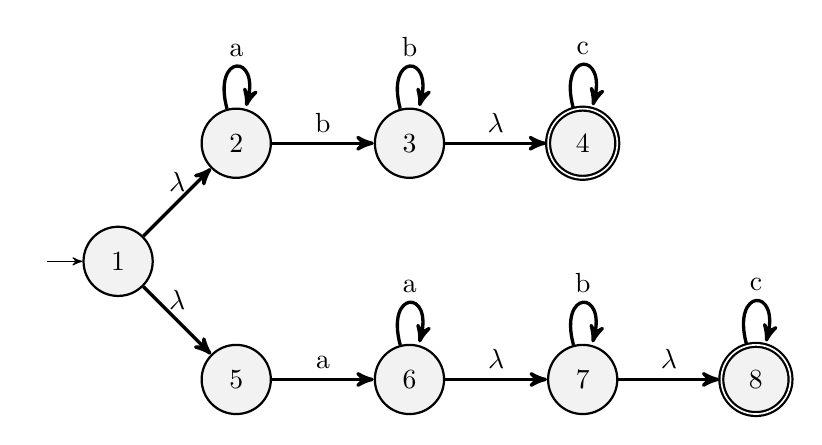
\begin{tikzpicture}[node distance=1.5cm]
    \node[state, initial] (1) {$1$};
    \node[state, above of=1, right of=1] (2) {$2$};
    \node[state, right of=2, xshift=7mm] (3) {$3$};
    \node[state, accepting, right of=3, xshift=7mm] (4) {$4$};
    \node[state, below of=1, right of=1] (5) {$5$};
    \node[state, right of=5, xshift=7mm] (6) {$6$};
    \node[state, right of=6, xshift=7mm] (7) {$7$};
    \node[state, accepting, right of=7, xshift=7mm] (8) {$8$};
    \draw[very thick]
      (1) edge[left, above] node{$\lambda$} (2)
      (1) edge[left, above] node{$\lambda$} (5)
      (2) edge[loop above] node{a} (2)
      (2) edge[left, above] node{b} (3)
      (3) edge[loop above] node{b} (3)
      (3) edge[left, above] node{$\lambda$} (4)
      (4) edge[loop above] node{c} (4)
      (5) edge[left, above] node{a} (6)
      (6) edge[loop above] node{a} (6)
      (6) edge[left, above] node{$\lambda$} (7)
      (7) edge[loop above] node{b} (7)
      (7) edge[left, above] node{$\lambda$} (8)
      (8) edge[loop above] node{c} (8);
  \end{tikzpicture}

\section{Question 6}
\noindent Consider the given NFA (1 is the start state) and its corresponding DFA (transition table) generated by applying the subset construction algorithm discussed in the class.\newline
  \begin{tabular}{|c|c|c|c|c|c|}
    \hline
	 \thead{Index} & \thead{State} & \thead{a} & \thead{b} & \thead{c} & \thead{Final?} \\
    \hline
	\textbf{1} & \{1,2,5\}   & \{2,6,7,8\} & \{3,4\}     & Err     & No \\
    \hline
	\textbf{2} & \{2,6,7,8\} & \{2,6,7,8\} & \{3,4,7,8\} & \{8\}   & Yes \\
    \hline
	\textbf{3} & \{3,4\}     & err         & \{3,4\}     & \{4\}   & Yes \\
    \hline
	\textbf{4} & \{3,4,7,8\} & err         & \{3,4,7,8\} & \{4,8\} & Yes \\
    \hline
	\textbf{5} & \{8\}       & err         & err         & \{8\}   & Yes \\
    \hline
	\textbf{6} & \{4\}       & err         & err         & \{4\}   & Yes \\
    \hline
	\textbf{7} & \{4,8\}     & err         & err         & \{4,8\} & Yes \\
    \hline
  \end{tabular}

\section{Question 7}
\noindent Consider the given DFA. Suppose that you use the algorithm discussed
in the class to further reduce it\newline
\begin{enumerate}
  \item How many states are in the \textit{reduced} DFA? \textbf{4} 
  \item How many Final states are in the \textit{reduced} DFA? \textbf{3}
\end{enumerate}
  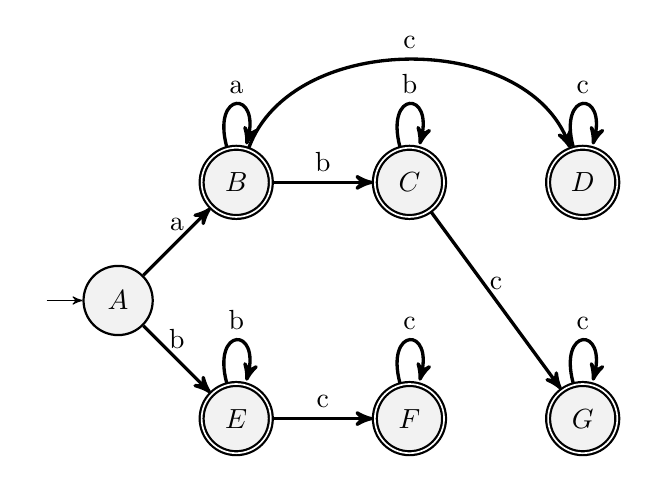
\begin{tikzpicture}[node distance=1.5cm]
    \node[state, initial] (1) {$A$};
    \node[state, accepting, above of=1, right of=1] (2) {$B$};
    \node[state, accepting, right of=2, xshift=7mm] (3) {$C$};
    \node[state, accepting, right of=3, xshift=7mm] (4) {$D$};
    \node[state, accepting, below of=1, right of=1] (5) {$E$};
    \node[state, accepting, right of=5, xshift=7mm] (6) {$F$};
    \node[state, accepting, right of=6, xshift=7mm] (7) {$G$};
    \draw[very thick]
      (1) edge[left, above] node{a} (2)
      (1) edge[left, above] node{b} (5)
      (2) edge[loop above] node{a} (2)
      (2) edge[left, above] node{b} (3)
      (2) edge[bend left=70, above] node{c} (4)
      (3) edge[loop above] node{b} (3)
      (3) edge[left, above] node{c} (7)
      (4) edge[loop above] node{c} (4)
      (5) edge[loop above] node{b} (5)
      (5) edge[left, above] node{c} (6)
      (6) edge[loop above] node{c} (6)
      (7) edge[loop above] node{c} (7);
  \end{tikzpicture}
  
\section{Question 8}
\noindent Consider the given DFA. Suppose that you use the algorithm discussed
in the class to further reduce it.\newline
\begin{enumerate}
  \item How many states are in the \textit{reduced} DFA? \textbf{4} 
  \item How many Final states are in the \textit{reduced} DFA? \textbf{3}
\end{enumerate}
  \begin{tabular}{|c|c|c|c|c|}
    \hline
	\thead{State} & \thead{a} & \thead{x} & \thead{y} & \thead{Final?} \\
    \hline
	\{1,2,3,4\} & \{3,5\}     & \{2,3,4\}   & \{4\}   & Yes \\
    \hline
	\{3,5\}     & \{3\}       & err         & err     & Yes \\
    \hline
	\{2,3,4\}   & \{3,5\}     & \{2,3,4\}   & \{4\}   & Yes \\
    \hline
	\{4\}       & \{5\}       & \{4\}       & \{4\}   & No \\
    \hline
	\{3\}       & \{3\}       & err         & err     & Yes \\
    \hline
	\{5\}       & err         & err         & err     & Yes \\
    \hline
  \end{tabular}


\renewcommand\thechapter{2}
\chapter{Top Down Parsing Lecture}

\section{First Sets}
First set ( beginning terminals) set of terminal and non-terminal, with empty string.
It is the first terminal in a production. If the first one contains lambda move to the next until last symbol or, no lambda or symbols. Top down uses leftmost derivation. We do not care about non-terminals - we want the set terminals!!!!!

\subsection{A Simple Example - Slides 4 - 15}
\vspace{-1.5em}
\begin{multicols}{2}
  \begin{enumerate}
    \setlength\itemsep{-.25em}
    \item S $\rightarrow$ ABc\$
    \item A $\rightarrow$ xaA
    \item A $\rightarrow$ yaA
    \item A $\rightarrow$ c
    \item B $\rightarrow$ b
    \item B $\rightarrow$ $\lambda$\newline\newline\newline\newline
  \end{enumerate}
  \setlength{\leftskip}{-12em}
  First (B) = First(b) $\cup$  First($\lambda$) = \textbf{ \{b, $\lambda$\}  $\leftarrow$ Final set of B}\newline
  First (A) = First(xaA) $\cup$ First(yaA) $\cup$ First(c)\newline
  \indent\hspace{2cm}2\hspace{5.5em}3\hspace{5.5em}4\newline
  \indent\hspace{.25cm}First (xaA) = First of \{x\} - $\lambda$ = \{x\} - $\lambda$ = \{x\}\newline
  \indent\hspace{.25cm}First (yaA) = First of \{y\} - $\lambda$ = \{y\} - $\lambda$ = \{y\}\newline
  \indent\hspace{.25cm}First (c) = \{c\}\newline
  First (A) = \{x\} $\cup$ \{y\} $\cup$ \{c\} = \textbf{ \{x, y, c\} $\leftarrow$ Final set of A}\newline
  First (S) = First(ABc\$) = \textbf{ \{x, y, c\} $\leftarrow$ Final set of S}
  \\
\end{multicols}

\vspace{-3em}

\subsection{Exercise - Slide 19}
\vspace{-1.5em}
\begin{multicols}{2}
  \begin{enumerate}
    \setlength\itemsep{-.25em}
    \item S $\rightarrow$ AB\$
    \item A $\rightarrow$ xaA
    \item A $\rightarrow$ yaA
    \item A $\rightarrow$ $\lambda$
    \item B $\rightarrow$ b\newline\newline\newline\newline
  \end{enumerate}
  \setlength{\leftskip}{-12em}
First (B) = First(b) = \textbf{ \{b\}  $\leftarrow$ Final set of B}\newline
First (A) = First(xaA) $\cup$  First(yaA) $\cup$  First($\lambda$)\newline
\indent\hspace{.25cm}First (xaA) = First of \{x\} - $\lambda$ = \{x\} - $\lambda$ = \{x\}\newline
\indent\hspace{.25cm}First (yaA) = First of \{y\} - $\lambda$ = \{x\} - $\lambda$ = \{y\}\newline
\indent\hspace{.25cm}First ($\lambda$) = First of {$\lambda$} - $\lambda$ = \{$\lambda$\}\newline
First (A) = First(x) $\cup$  First(y) $\cup$  First($\lambda$)\newline
First (A) = \{x\} $\cup$  \{y\} $\cup$  \{$\lambda$\} = \textbf{ \{x, y, $\lambda$\} $\leftarrow$ Final set of A}\newline
First (S) = First(AB\$) = (First(A) - $\lambda$) $\cup$ (\{b\} - $\lambda$) = \textbf{\{x, y, b\} $\leftarrow$ Final set S}
\end{multicols}
\vspace{-1em}
\noindent\textbf{note:} *First of $\lambda$ is $\lambda$* -
First($\lambda$) = (First($\lambda$) - $\lambda$) = {$\lambda$} "reading $\lambda$" 

\subsection{In Class Quiz Q5 - Slide 25}
\vspace{-1.5em}
\begin{multicols}{2}
  \begin{enumerate}
    \setlength\itemsep{-.25em}
    \item S $\rightarrow$ AA\$
    \item A $\rightarrow$ xAy
    \item A $\rightarrow$ BB
    \item B $\rightarrow$ zB
    \item B $\rightarrow$ q\newline
  \end{enumerate}
  \setlength{\leftskip}{-12em}
First (B) = First(zB) $\cup$ First(q) = \textbf{ \{z, q\}  $\leftarrow$ Final set of B}\newline
First (A) = First(xAy) \newline
\indent\hspace{1cm}= \{x\} $\cup$ \{z\} $\cup$ \{q\} = \textbf{ \{x, z, q\} $\leftarrow$ Final set of A}\newline
First (S) = \{x\} $\cup$ \{z\} $\cup$ \{q\} = \textbf{ \{x, z, q\} $\leftarrow$ Final set of S}\newline
\{z, q\}, \{x, z, q\} and \{x, z, q\}
\end{multicols}
\vspace{-1em}
\noindent\textbf{note:} you could have a \$ if it is the first, like $\lambda$\newline
\indent\hspace{.5cm}first sets are needed for everything, it will mess up parse table without

\section{Follow Sets}
\textbf{NO LAMBDA'S EVER!!!!}
All production beginning on the right hand side\newline
Follow set of S is the empty set
 - represents the entire string, so it will never have anything following!!!!

\subsection{Exercise - Slide 28}
\vspace{-1.5em}
\begin{multicols}{2}
  \begin{enumerate}
    \setlength\itemsep{-.25em}
    \item S $\rightarrow$ AB\$
    \item A $\rightarrow$ xaA
    \item A $\rightarrow$ yaA
    \item A $\rightarrow$ $\lambda$
    \item B $\rightarrow$ b\newline\newline
  \end{enumerate}
  \setlength{\leftskip}{-12em}
Follow (S) = \textbf{ \{\} $\leftarrow$ Final set of S}\newline
Follow (B) = First(\$) = \textbf{ \{\$\}  $\leftarrow$ Final set of B}\newline
Follow (A) = First(B\$) $\cup$ Follow(A) $\cup$ Follow (A)\newline
\indent\hspace{.25cm}(First(B) - $\lambda$) = \{b\}\newline
\indent\hspace{.25cm}First(B\$) = \{b\}\newline
Follow (A) = \{b\} = \textbf{ \{b\} $\leftarrow$ Final set of A}\newline
\end{multicols}

\subsection{In Class Quiz Q6 - Slide 30}
\vspace{-1em}
\begin{multicols}{2}
  \begin{enumerate}
    \setlength\itemsep{-.25em}
    \item S $\rightarrow$ AA\$
    \item A $\rightarrow$ xAy
    \item A $\rightarrow$ BB
    \item B $\rightarrow$ zB
    \item B $\rightarrow$ q\newline\newline\newline
  \end{enumerate}
  \setlength{\leftskip}{-12em}
Follow (S) = \textbf{ \{\} $\leftarrow$ Final set of S}\newline
Follow (A) = First(A\$) $\cup$ First(\$) $\cup$ First (y)\newline
\indent\hspace{1.25cm}= (First(A) - $\lambda$) $\cup$ \{\$\} $\cup$ \{y\}\newline
\indent\hspace{1.25cm}= \{x, z, q\} $\cup$ \{\$\} $\cup$ {y}\newline
\indent\hspace{1.25cm}= \textbf{ \{x, z, q, y, \$\} $\leftarrow$ Final set of A}\newline
Follow (B) = First (B) $\cup$ Follow(A) $\cup$ \st{Follow (B)} $\leftarrow$ CROSS OUT FOLLOW(B)\newline
\indent\hspace{1.25cm}= \{z, q\} $\cup$ Follow(A)\newline
\indent\hspace{1.25cm}= \textbf{ \{x, z, q, y, \$\} $\leftarrow$ Final set of B}
\end{multicols}
\vspace{-1em}
%\textbf{MAKE SURE TO SHOW ALL WORK} including crossing out follows, etc

\subsection{A Simple Example - Slides 4 - 15 - Follow Set}
\vspace{-1em}
\begin{multicols}{2}
  \begin{enumerate}
    \setlength\itemsep{-.25em}
    \item S $\rightarrow$ ABc\$
    \item A $\rightarrow$ xaA
    \item A $\rightarrow$ yaA
    \item A $\rightarrow$ c
    \item B $\rightarrow$ b
    \item B $\rightarrow$ $\lambda$\newline
  \end{enumerate}
  \setlength{\leftskip}{-12em}
Follow (S) = \textbf{ \{\} $\leftarrow$ Final set of S}\newline
Follow (A) = First(Bc) $\cup$ \st{Follow(A) $\cup$ Follow(A)}\newline
\indent\hspace{1.25cm}= (First(B) - $\lambda$) $\cup$ First(c)\newline
\indent\hspace{1.25cm}= \{b\} $\cup$ \{c\} = \textbf{ \{b, c\} $\leftarrow$ Final set of A}\newline
Follow (B) = \textbf{ \{c\} $\leftarrow$ Final set of B}\newline  
\end{multicols}


\section{Predict Sets}
\subsection{Exercise - Slide 32}
\vspace{-1em}
\begin{multicols}{2}
  \begin{enumerate}
    \setlength\itemsep{-.25em}
    \item S $\rightarrow$ AB\$
    \item A $\rightarrow$ xaA
    \item A $\rightarrow$ yaA
    \item A $\rightarrow$ $\lambda$
    \item B $\rightarrow$ b
  \end{enumerate}
  parse table LL(1) \textbf{abxy\$}\newline
  \begin{tabular}{|c|c|c|c|c|c|}
    \hline
	  & \thead{a} & \thead{b} & \thead{x} & \thead{y} & \thead{\$}\\
    \hline
	\textbf{S} &  & 1 & 1 & 1 & \\
    \hline
	\textbf{A} &  & 4 & 2 & 3 & \\
    \hline
	\textbf{B} &  & 5 &   &   & \\
    \hline
  \end{tabular}
  \newline\newline\newline\newline\newline
  
\setlength{\leftskip}{-12em}
\hspace{-.5cm}Predict(1 S $\rightarrow$ AB\$) = \{x, y, b\}\newline
\indent\hspace{.25cm}First (B) = First(b) = \textbf{ \{b\} $\leftarrow$ Final set of B}\newline
\indent\hspace{.25cm}First (A) = First(xaA) $\cup$  First(yaA) $\cup$  First($\lambda$) (from slide 19)\newline
\indent\hspace{1cm}First (xaA) = First of \{x\} - $\lambda$ = \{x\} - $\lambda$ = \{x\}\newline
\indent\hspace{1cm}First (yaA) = First of \{y\} - $\lambda$ = \{x\} - $\lambda$ = \{y\}\newline
\indent\hspace{1cm}First ($\lambda$) = First of \{$\lambda$\} - $\lambda$ = \{$\lambda$\}\newline
\indent\hspace{1cm}First (A) = First(x) $\cup$  First(y) $\cup$  First($\lambda$)\newline
\indent\hspace{1cm}First (A) = \{x\} $\cup$ \{y\} $\cup$  \{$\lambda$\} = \textbf{ \{x, y, $\lambda$\} $\leftarrow$ Final set of A}\newline
\indent\hspace{.25cm}First(AB\$) = (First(A) - $\lambda$) $\cup$ First(B) = \textbf{ \{x, y, b\}$\leftarrow$ Final set of AB\$} \newline
Predict(1. A $\rightarrow$ AB\$) = \textbf{\{x, y, b\} $\leftarrow$ Final}\newline
Predict(2. A $\rightarrow$ xaA) = \textbf{\{x\} $\leftarrow$ Final}\newline
Predict(3. A $\rightarrow$ yaA) = \textbf{\{y\} $\leftarrow$ Final}\newline
Predict(4. A $\rightarrow$ $\lambda$) = (First($\lambda$) - $\lambda$) $\cup$ Follow(A)				(from slide 28)\newline
\indent\hspace{2.3cm}= \textbf{\{b\} Final}\newline
Predict(5. B $\rightarrow$ b) = \textbf{\{b\} Final}
\end{multicols}

\subsection{An Example - Slide 36-37}
Stack-based parser for LL(1) \textbf{xayab\$}\newline
\begin{tabular}{|c|c|c|}
\hline
	\thead{Parse stack} & \thead{Remaining Input} & \thead{Parser action}\\
\hline
	S       & xayab\$ & predict 1\\
\hline
	AB\$   & xayab\$ & predict 2\\
\hline
	xaAB\$ & xayab\$ & match(x)\\
\hline
	aAB\$  & ayab\$   & match(a)\\
\hline
	AB\$  & yab\$   & predict 3\\
\hline
	yaAB\$ & yab\$   & match(y)\\
\hline
	aAB\$  & ab\$    & match(a)\\
\hline
	AB\$   & b\$     & predict 4\\
\hline
	B\$    & b\$    & predict 5\\
\hline
	b\$    & b\$    & match(b)\\
\hline
	\$     & \$     & done\\
\hline
\end{tabular}

\newpage
\subsection{In Class Quiz Q11 - Slide 43}
\vspace{-1em}
\begin{multicols}{2}
  \begin{enumerate}
    \setlength\itemsep{-.25em}
    \item S $\rightarrow$ AA\$
    \item A $\rightarrow$ xAy
    \item A $\rightarrow$ BB
    \item B $\rightarrow$ zB
    \item B $\rightarrow$ q\newline\newline
  \end{enumerate}
  \setlength{\leftskip}{-12em}
  predict(1. S $\rightarrow$ AA\$) = First(AA\$) = \textbf{ \{x, z, q\} $\leftarrow$ Final}\newline
  predict(2. A $\rightarrow$ xAy\$) = \textbf{ \{x\} $\leftarrow$ Final}\newline
  predict(3. A $\rightarrow$ BB\$) = \textbf{ \{z, q\} $\leftarrow$ Final}\newline
  predict(4. B $\rightarrow$ zB\$) = \textbf{ \{z\} $\leftarrow$ Final}\newline
  predict(5. B $\rightarrow$ q\$) = \textbf {\{q\} $\leftarrow$ Final}\newline
\end{multicols}
\vspace{-1em}
\noindent\textbf{parser table ll(1)}\newline
  \begin{tabular}{|c|c|c|c|c|c|}
    \hline
	  & \thead{q} & \thead{x} & \thead{y} & \thead{z} & \thead{\$}\\
    \hline
	\textbf{S} & 1 & 1 &   & 1 & \\
    \hline
	\textbf{A} & 3 & 2 &   & 3 & \\
    \hline
	\textbf{B} & 5 &   &   & 4 & \\
    \hline
  \end{tabular}
  
\subsection{A Simple Example - Slides 4 - 15 - Predict Set}
\vspace{-1em}
\begin{multicols}{2}
  \begin{enumerate}
    \setlength\itemsep{-.25em}
    \item S $\rightarrow$ ABc\$
    \item A $\rightarrow$ xaA
    \item A $\rightarrow$ yaA
    \item A $\rightarrow$ c
    \item B $\rightarrow$ b
    \item B $\rightarrow$ $\lambda$\newline\newline
  \end{enumerate}
  \setlength{\leftskip}{-12em}
  predict(1. S $\rightarrow$ ABc\$) = \textbf{ \{x, y, c\} $\leftarrow$ Final}\newline
  predict(2. A $\rightarrow$ xaA) = \textbf{ \{x\} $\leftarrow$ Final}\newline
  predict(3. A $\rightarrow$ yaA\$) = \textbf{ \{y\} $\leftarrow$ Final}\newline
  predict(4. A $\rightarrow$ c\$) = \textbf{ \{c\} $\leftarrow$ Final}\newline
  predict(5. B $\rightarrow$ b\$) = \textbf{ \{b\} $\leftarrow$ Final}\newline
  predict(6. B $\rightarrow$ $\lambda$\$) = \textbf {\{c\} $\leftarrow$ Final}\newline
\end{multicols}
\vspace{-1em}
\noindent\textbf{parser table ll(1)}\newline
  \begin{tabular}{|c|c|c|c|c|c|}
    \hline
	  & \thead{b} & \thead{c} & \thead{x} & \thead{y} & \thead{\$}\\
    \hline
	\textbf{S} &   & 1 & 1 & 1 & \\
    \hline
	\textbf{A} &   & 4 & 2 & 3 & \\
    \hline
	\textbf{B} & 5 & 6 &   &   & \\
    \hline
  \end{tabular}

\newpage
\renewcommand\thechapter{Q2}
\chapter{Take Home Quiz 2}
\section{Question 2}
  \begin{enumerate}
    \setlength\itemsep{-.25em}
    \renewcommand{\labelenumii}{\arabic{enumii}.}
    \item E $\rightarrow$ Prefix (E)
    \item E $\rightarrow$ V Tail
    \item Prefix $\rightarrow$ F
    \item Prefix $\rightarrow$ $\lambda$
    \item Tail $\rightarrow$ + E
    \item Tail $\rightarrow$ $\lambda$
  \end{enumerate}
\setlength{\leftskip}{1em}
\textbf{False - Parse tree for "F(V + V + V)" using LMD is not equal to that of RMD}\newline
Parse trees are the same regardless of LMD or RMD, but the derivations are different\newline

\noindent\{(), V, F, +, $\lambda$\} = \textbf{5 terminals} \{E, Prefix, Tail\} = \textbf{3 non-terminals} and \textbf{6 productions}\newline

\noindent\textbf{LMD}\newline
E $\rightarrow$ Prefix (E) $\rightarrow$ F(E) $\rightarrow$ F(V Tail) $\rightarrow$ F(V + E)
$\rightarrow$ F(V + V Tail) $\rightarrow$ F(V + V + E)\newline
\indent\hspace{-.2cm}$\rightarrow$ F(V + V + V Tail) $\rightarrow$ F(V + V + V $\lambda$)
$\rightarrow$ \textbf{F(V + V + V)}\newline

\noindent\textbf{RMD}\newline
E $\rightarrow$ Prefix (E) $\rightarrow$ Prefix(V Tail) $\rightarrow$ Prefix(V + E)
$\rightarrow$ Prefix(V + V Tail) $\rightarrow$ Prefix(V + V + E)\newline
\indent\hspace{-.2cm}$\rightarrow$ Prefix(V + V + V Tail) $\rightarrow$ Prefix(V + V + V $\lambda$))
$\rightarrow$ Prefix(V + V + V) $\rightarrow$ \textbf{F(V + V + V)}\newline
\vspace{-1em}
\subsection{F(V + V +)}
\noindent\textbf{LMD}\newline
E $\rightarrow$ Prefix (E) $\rightarrow$ F(E) $\rightarrow$ F(V Tail) $\rightarrow$ F(V + E)
$\rightarrow$ F(V + V Tail) $\rightarrow$ F(V + V + E) \textbf{$\leftarrow$ error}\newline
Cannot replace E with $\lambda$\newline

\noindent\textbf{RMD}\newline
E $\rightarrow$ Prefix (E) $\rightarrow$ Prefix(V Tail) $\rightarrow$ Prefix(V + E)
$\rightarrow$ Prefix(V + V Tail) $\rightarrow$ Prefix(V + V + E) \textbf{$\leftarrow$ error}\newline
Cannot replace E with $\lambda$

\newpage
\section{Question 3 - First set of A}
\vspace{-1em}
\begin{multicols}{2}
  \begin{enumerate}
    \setlength\itemsep{-.25em}
    \item S $\rightarrow$ AB\$
    \item A $\rightarrow$ xaA
    \item A $\rightarrow$ yaA
    \item A $\rightarrow$ $\lambda$
    \item B $\rightarrow$ b
    \item B $\rightarrow$ A\newline
  \end{enumerate}
\setlength{\leftskip}{-12em}
First (A) = First(xaA) $\cup$  First(yaA) $\cup$  First($\lambda$)\newline
\indent\hspace{.25cm}First (xaA) = First of \{x\} - $\lambda$ = \{x\} - $\lambda$ = \{x\}\newline
\indent\hspace{.25cm}First (yaA) = First of \{y\} - $\lambda$ = \{x\} - $\lambda$ = \{y\}\newline
\indent\hspace{.25cm}First ($\lambda$) = First of {$\lambda$} - $\lambda$ = \{$\lambda$\}\newline
First (A) = First(x) $\cup$  First(y) $\cup$  First($\lambda$)\newline
First (A) = \{x\} $\cup$  \{y\} $\cup$  \{$\lambda$\} = \textbf{\{x, y, $\lambda$\} $\leftarrow$ Final set of A}
\end{multicols}

\section{Question 4 - First set of B}
\vspace{-1em}
\begin{multicols}{2}
  \begin{enumerate}
    \setlength\itemsep{-.25em}
    \item S $\rightarrow$ AB\$
    \item A $\rightarrow$ xaA
    \item A $\rightarrow$ yaA
    \item A $\rightarrow$ $\lambda$
    \item B $\rightarrow$ b
    \item B $\rightarrow$ A\newline
  \end{enumerate}
\setlength{\leftskip}{-12em}
First (B) = First(b) $\cup$  First(A) = \textbf{\{b, x, y, $\lambda$\}  $\leftarrow$ Final set of B}\newline
\newline\newline\newline\newline
\end{multicols}

\vspace{-3em}
\section{Question 5 - First set of S}
\vspace{-1em}
\begin{multicols}{2}
  \begin{enumerate}
    \setlength\itemsep{-.25em}
    \item S $\rightarrow$ AB\$
    \item A $\rightarrow$ xaA
    \item A $\rightarrow$ yaA
    \item A $\rightarrow$ $\lambda$
    \item B $\rightarrow$ b
    \item B $\rightarrow$ A
  \end{enumerate}
\setlength{\leftskip}{-12em}
First (S) = First(AB\$) = (First(A) - $\lambda$) $\cup$ (First(B) - $\lambda$) $\cup$ (First(\$) - $\lambda$)\newline
\indent\hspace{.75cm} = \textbf{\{x, y, b, \$\} $\leftarrow$ Final set of S}
\newline\newline\newline
\end{multicols}

\vspace{-1.5em}
\section{Question 6 - Follow set of B}
\vspace{-1em}
\begin{multicols}{2}
  \begin{enumerate}
    \setlength\itemsep{-.25em}
    \item S $\rightarrow$ AB\$
    \item A $\rightarrow$ xaA
    \item A $\rightarrow$ yaA
    \item A $\rightarrow$ $\lambda$
    \item B $\rightarrow$ b
    \item B $\rightarrow$ A
  \end{enumerate}
\setlength{\leftskip}{-12em}
Follow (B) = First(\$) = \textbf{\{\$\}  $\leftarrow$ Final set of B}
\newline\newline\newline\newline
\end{multicols}

\vspace{-1.5em}
\section{Question 7 - Follow set of A}
\vspace{-1em}
\begin{multicols}{2}
  \begin{enumerate}
    \setlength\itemsep{-.25em}
    \item S $\rightarrow$ AB\$
    \item A $\rightarrow$ xaA
    \item A $\rightarrow$ yaA
    \item A $\rightarrow$ $\lambda$
    \item B $\rightarrow$ b
    \item B $\rightarrow$ A\newline\newline
  \end{enumerate}
\setlength{\leftskip}{-12em}
Follow (A) = First(B\$) $\cup$ Follow(A) $\cup$ Follow (A)\newline
First (B) = First(b) $\cup$  First(A) = \{b, x, y, $\lambda$\}  $\leftarrow$ \textbf{Final set of B}\newline
\indent\hspace{.25cm}(First(B) - $\lambda$) = \{b, x, y\}\newline
\indent\hspace{.25cm}First(B\$) = First(B) $\cup$ First(\$) =\{b, x, y, \$\}\newline
Follow (A) = \{b, x, y, \$\} = \textbf{\{b, x, y, \$\} $\leftarrow$ Final set of A}\newline
\newline
\end{multicols}

\vspace{-3em}
\section{Questions 8 - 10}
\vspace{-1.5em}
\begin{multicols}{2}
  \begin{enumerate}
    \setlength\itemsep{-.25em}
    \item S $\rightarrow$ AB\$
    \item A $\rightarrow$ xaA
    \item A $\rightarrow$ yaA
    \item A $\rightarrow$ $\lambda$
    \item B $\rightarrow$ b
    \item B $\rightarrow$ A\newline\newline\newline\newline\newline\newline\newline\newline\newline\newline\newline
  \end{enumerate}
\setlength{\leftskip}{-12em}
Predict(1 S $\rightarrow$ AB\$) = \textbf{\{x, y, b, \$\} $\leftarrow$ Predict 1}\newline
\indent\hspace{.25cm}First (B) = First(b) = \textbf{ \{b\} $\leftarrow$ Final set of B}\newline
\indent\hspace{.25cm}First (A) = First(xaA) $\cup$  First(yaA) $\cup$  First($\lambda$) (from slide 19)\newline
\indent\hspace{1cm}First (xaA) = First of \{x\} - $\lambda$ = \{x\} - $\lambda$ = \{x\}\newline
\indent\hspace{1cm}First (yaA) = First of \{y\} - $\lambda$ = \{x\} - $\lambda$ = \{y\}\newline
\indent\hspace{1cm}First ($\lambda$) = First of \{$\lambda$\} - $\lambda$ = \{$\lambda$\}\newline
\indent\hspace{1cm}First (A) = First(x) $\cup$  First(y) $\cup$  First($\lambda$)\newline
\indent\hspace{1cm}First (A) = \{x\} $\cup$ \{y\} $\cup$  \{$\lambda$\} = \textbf{ \{x, y, $\lambda$\} $\leftarrow$ Final set of A}\newline
\indent\hspace{.25cm}First(AB\$) = (First(A) - $\lambda$) $\cup$ First(B) = \textbf{ \{x, y, b\}$\leftarrow$ Final set of AB\$} \newline
Predict(1 S $\rightarrow$ AB\$) = \textbf{\{x, y, b, \$\} $\leftarrow$ Predict 1}\newline
Predict(2 A $\rightarrow$ xaA) = \textbf{ \{x\} $\leftarrow$ Predict 2}\newline
Predict(3 A $\rightarrow$ yaA) = \textbf{ \{y\} $\leftarrow$ Predict 3}\newline
Predict(4 A $\rightarrow$ $\lambda$) = (First($\lambda$) - $\lambda$) $\cup$ Follow(A)\newline
\indent\hspace{2.3cm}= \textbf{\{b, x, y, \$\} $\leftarrow$ Predict 4}\newline
Predict(5 B $\rightarrow$ b) = \textbf{\{b\} $\leftarrow$ Predict 5}\newline
Predict(6 B $\rightarrow$ A) = (First(A) - $\lambda$) $\cup$ Follow(B)\ = \textbf{\{x, y, \$\} $\leftarrow$ Predict 6}
\end{multicols}

\section{Question 8 - Predict(1)}
\hspace{-.3cm}Predict(1 S $\rightarrow$ AB\$) = \textbf{\{x, y, b, \$\} $\leftarrow$ Predict 1}

\section{Question 9 - Predict(4)}
\hspace{-.3cm}Predict(4 A $\rightarrow$ $\lambda$) = (First($\lambda$) - $\lambda$) $\cup$ Follow(A)\ = \textbf{\{b, x, y, \$\} $\leftarrow$ Predict 4}

\section{Question 10 - Predict(6)}
\hspace{-.3cm}Predict(6 B $\rightarrow$ A) = (First(A) - $\lambda$) $\cup$ Follow(B)\ = \textbf{\{x, y, \$\} $\leftarrow$ Predict 6}

\section{Question 11 - Parse Table LL(1)}
  \begin{tabular}{|c|c|c|c|c|c|}
    \hline
	 & \thead{a} & \thead{b} & \thead{x} & \thead{y} & \thead{\$}\\
    \hline
	\textbf{S} &  & 1 & 1 & 1 & 1\\
    \hline
	\textbf{A} &  & 4 & 2,4 & 3,4 & 4\\
    \hline
	\textbf{B} &  & 5 & 6  & 6 & 6 \\
    \hline
\end{tabular}

\section{Question 12 - Parse Table LL(1)}
\vspace{-1.5em}
\begin{multicols}{2}
  \begin{enumerate}
    \setlength\itemsep{-.25em}
    \item S $\rightarrow$ AB\$
    \item A $\rightarrow$ xaA
    \item A $\rightarrow$ yaA
    \item A $\rightarrow$ $\lambda$
    \item B $\rightarrow$ b
  \end{enumerate}
  Parse table LL(1)\newline
  \begin{tabular}{|c|c|c|c|c|c|}
    \hline
	  & \thead{a} & \thead{b} & \thead{x} & \thead{y} & \thead{\$}\\
    \hline
	\textbf{S} &  & 1 & 1 & 1 & \\
    \hline
	\textbf{A} &  & 4 & 2 & 3 & \\
    \hline
	\textbf{B} &  & 5 &   &   & \\
    \hline
\end{tabular}
\end{multicols}

Stack-based parser for LL(1) \textbf{yaxa\$}\newline
\begin{tabular}{|c|c|c|}
\hline
	\thead{Parse stack} & \thead{Remaining Input} & \thead{Parser action}\\
\hline
	S      & yaxa\$ & predict 1\\
\hline
	AB\$   & yaxa\$ & predict 3\\
\hline
	yaAB\$ & yaxa\$ & match(y)\\
\hline
	aAB\$  & axa\$  & match(a)\\
\hline
	AB\$   & xa\$   & predict 2\\
\hline
	xaAB\$ & xa\$   & match(x)\\
\hline
	aAB\$  & a\$    & match(a)\\
\hline
	AB\$   & \$     & error\\
\hline
\end{tabular}

\renewcommand\thechapter{3}
\chapter{Bottom Up Parsing - Lecture 3 : 2-14-2022}
\section{LR Parsers}
\subsection{Configuration Closure Set}
Closure set - ( { S → .E\$} )

State 0
 = \{ S $\leftarrow$ \textbf{.}E\$, E $\leftarrow$ \textbf{.}E + T, E $\leftarrow$ \textbf{.}T, T $\leftarrow$ \textbf{.}ID, T $\leftarrow$ \textbf{.}(E) \}

\section{Characterstic Finite State Machine}
\vspace{-1.5em}  
\begin{multicols}{3}
\subsection{Example - Slide 11}
\noindent
  \begin{enumerate}
    \setlength\itemsep{-.25em}
    \item S' $\rightarrow$ S\$
    \item S $\rightarrow$ ID\newline\newline\newline\newline\newline\newline\newline
  \end{enumerate}
\subsubsection{State Diagram}
\noindent
  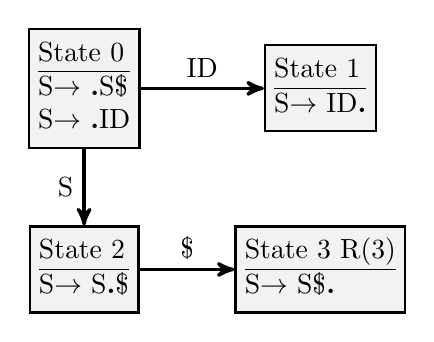
\begin{tikzpicture}
    \node[state, shape=rectangle] (0) {
    \makecell[l] {
    State 0 \\
    \hline
    S$\rightarrow$ \textbf{.}S\$ \\
    S$\rightarrow$ \textbf{.}ID
    }};
    \node[state, shape=rectangle, right of=0] (1) {
    \makecell[l] {
    State 1 \\
    \hline
    S$\rightarrow$ ID\textbf{.} \\
    }};
    \node[state, shape=rectangle, below of=0, yshift=7mm] (2) {
    \makecell[l] {
    State 2 \\
    \hline
    S$\rightarrow$ S\textbf{.}\$ \\
    }};
    \node[state, shape=rectangle, below of=1, yshift=7mm] (3) {
    \makecell[l] {
    State 3 R(3)\\
    \hline
    S$\rightarrow$ S\$\textbf{.}
    }};
    \draw[very thick]
          (0) edge[right, above] node{ID} (1)
          (0) edge[right, left] node{S} (2)
          (2) edge[right, above] node{\$} (3);
  \end{tikzpicture}
\subsubsection{GoTo/Action Table}
  \begin{tabular}{|c|c|c|c|c|c|}
    \hline
	  & \multicolumn{3}{c|}{Symbol} & Action Table\\
    \hline
	  & \thead{ID} & \thead{\$} & \thead{S} & \thead{Action}\\
    \hline
	\textbf{0} & 1 &   & 2 & Shift\\
    \hline
	\textbf{1} &   &   &   & Reduce 2\\
    \hline
	\textbf{2} &   & 3 &   & Shift\\
    \hline
	\textbf{3} &   &   &   & Accept R(1)\\
    \hline
  \end{tabular}
\end{multicols}


\subsection{Simple Example - Slide 13 or 20}
\vspace{-1.5em}  
\begin{multicols}{2}
\subsubsection{State Diagram}
\noindent
  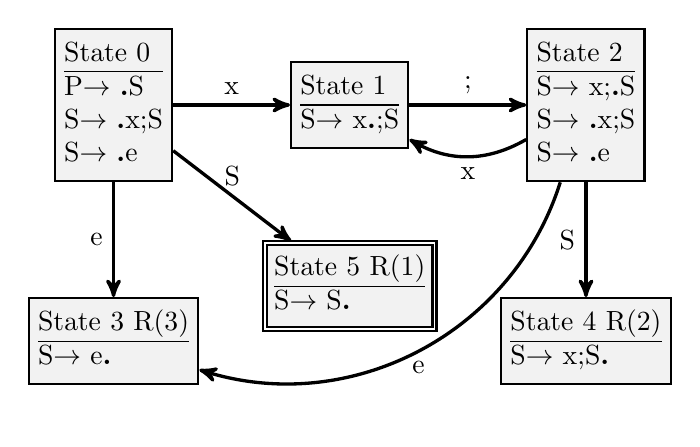
\begin{tikzpicture}
    \node[state, shape=rectangle] (0) {
    \makecell[l] {
    State 0 \\
    \hline
    P$\rightarrow$ \textbf{.}S \\
    S$\rightarrow$ \textbf{.}x;S \\
    S$\rightarrow$ \textbf{.}e
    }};
    \node[state, shape=rectangle, right of=0] (1) {
    \makecell[l] {
    State 1 \\
    \hline
    S$\rightarrow$ x\textbf{.};S \\
    }};
    \node[state, shape=rectangle, right of=1] (2) {
    \makecell[l] {
    State 2 \\
    \hline
    S$\rightarrow$ x;\textbf{.}S \\
    S$\rightarrow$ \textbf{.}x;S \\
    S$\rightarrow$ \textbf{.}e
    }};
    \node[state, shape=rectangle, below of=0] (3) {
    \makecell[l] {
    State 3 R(3)\\
    \hline
    S$\rightarrow$ e\textbf{.}
    }};
    \node[state, shape=rectangle, below of=2] (4) {
    \makecell[l] {
    State 4 R(2) \\
    \hline
    S$\rightarrow$ x;S\textbf{.} \\
    }};
    \node[state, accepting, shape=rectangle, below of=1, yshift=7mm] (5) {
    \makecell[l] {
    State 5 R(1) \\
    \hline
    S$\rightarrow$ S\textbf{.} \\
    }};
    \draw[very thick]
          (0) edge[right, above] node{x} (1)

          (0) edge[right, left] node{e} (3)
          (0) edge[right, above] node{S} (5)
          (1) edge[right, above] node{;} (2)
          (2) edge[bend left, below] node{x} (1)
          (2) edge[bend left=45, below] node{e} (3)
          (2) edge[right, left] node{S} (4);
  \end{tikzpicture}
\subsubsection{GoTo/Action Table}
  \begin{tabular}{|c|c|c|c|c|c|c|c|}
    \hline
	  & \multicolumn{5}{c|}{Symbol} & Action Table\\
    \hline
	  & \thead{x} & \thead{;} & \thead{e} & \thead{P} & \thead{S} & \thead{Action}\\
    \hline
	\textbf{0} & 1 &   & 3 &   & 5 & Shift\\
    \hline
	\textbf{1} &   & 2 &   &   &   & Shift\\
    \hline
	\textbf{2} & 1 &   & 3 &   & 4 & Shift\\
    \hline
	\textbf{3} &   &   &   &   &   & Reduce 3\\
    \hline
	\textbf{4} &   &   &   &   &   & Reduce 2\\
    \hline
	\textbf{5} &   &   &   &   &   & Accept R(1)\\
    \hline
  \end{tabular}
  \newline\newline
\end{multicols}

\vspace{-2.5em}
\begin{multicols}{2}
\subsubsection{Parser Table for String x;x;e}
\noindent
  \begin{tabular}{|c|c|c|c|}
    \hline
	\thead{} & \thead{Parse Stack} & \thead{Remaining} & \thead{Parser Action}\\
    \hline
	\textbf{1} & 0      & x;x;e & Shift 1 \\
    \hline
	\textbf{2} & 01     & ;x;e  & Shift 2 \\
    \hline
	\textbf{3} & 012    & x;e   & Shift 1 \\
    \hline
	\textbf{4} & 0121   & ;e    & Shift 2 \\
    \hline
	\textbf{5} & 01212  & e     & Shift 3 \\
    \hline
	\textbf{6} & 012123 &       & R(3) Goto State 4  \\
    \hline
	\textbf{7} & 012124 &       & R(2) Goto State 4  \\
    \hline
	\textbf{8} & 0124   &       & R(2) Goto State 5  \\
    \hline
	\textbf{9} & 05     &       & Accept State  \\
    \hline
  \end{tabular}
  \newline\newline
  \subsubsection{Parser Table for String x;x;x;e}
  \begin{tabular}{|c|c|c|c|}
    \hline
	\thead{} & \thead{Parse Stack} & \thead{Remaining} & \thead{Parser Action}\\
    \hline
	\textbf{1}  & 0        & x;x;x;e & Shift 1 \\
    \hline
	\textbf{2}  & 01       & ;x;x;e  & Shift 2 \\
    \hline
	\textbf{3}  & 012      & x;x;e   & Shift 1 \\
    \hline
	\textbf{4}  & 0121     & ;x;e    & Shift 2 \\
    \hline
	\textbf{5}  & 01212    & x;e     & Shift 1 \\
    \hline
	\textbf{6}  & 012121   & ;e      & Shift 2 \\
    \hline
	\textbf{7}  & 0121212  & e       & Shift 3 \\
    \hline
	\textbf{8}  & 01212123 &         & R(3) Goto State 4  \\
    \hline
	\textbf{9}  & 01212124 &         & R(2) Goto State 4  \\
    \hline
	\textbf{10} & 012124   &         & R(2) Goto State 4  \\
    \hline
	\textbf{11} & 0124     &         & R(2) Goto State 5  \\
    \hline
	\textbf{12} & 05       &         & Accept State  \\
    \hline
  \end{tabular}
\end{multicols}

\subsection{Shift Reduce conflict}
\vspace{-1.5em}
\begin{multicols}{2}
  \begin{enumerate}
    \setlength\itemsep{-.25em}
    \item S $\rightarrow$ Ay
    \item A $\rightarrow$ x
    \item A $\rightarrow$ xx\newline\newline\newline\newline\newline\newline\newline\newline\newline\newline\newline\newline
  \end{enumerate}
  \vspace{-80pt}
  \setlength{\leftskip}{-10em}
  \subsubsection{State Diagram}
  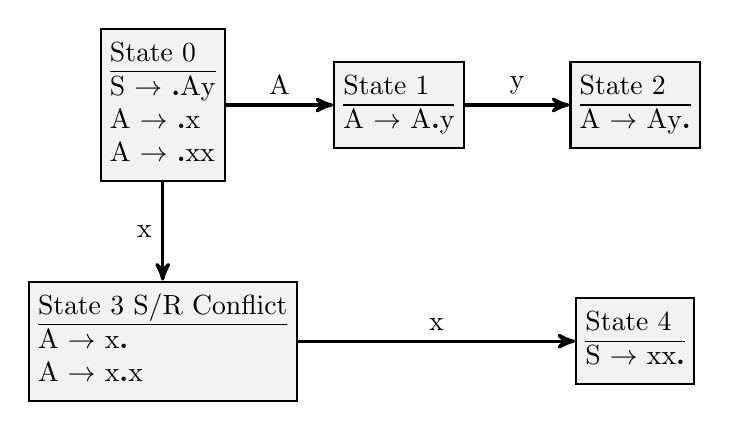
\begin{tikzpicture}
    \node[state, shape=rectangle] (0) {
    \makecell[l] {
    State 0 \\
    \hline
    S $\rightarrow$ \textbf{.}Ay \\
    A $\rightarrow$ \textbf{.}x \\
    A $\rightarrow$ \textbf{.}xx
    }};
    \node[state, shape=rectangle, right of=0] (1) {
    \makecell[l] {
    State 1 \\
    \hline
    A $\rightarrow$ A\textbf{.}y
    }};
    \node[state, shape=rectangle, right of=1] (2) {
    \makecell[l] {
    State 2 \\
    \hline
    A $\rightarrow$ Ay\textbf{.}
    }};
    \node[state, shape=rectangle, below of=0] (3) {
    \makecell[l] {
    State 3 S/R Conflict\\
    \hline
    A $\rightarrow$ x\textbf{.} \\
    A $\rightarrow$ x\textbf{.}x
    }};
    \node[state, shape=rectangle, below of=2] (4) {
    \makecell[l] {
    State 4 \\
    \hline
    S $\rightarrow$ xx\textbf{.} \\
    }};
    \draw[very thick]
          (0) edge[right, above] node{A} (1)
          (0) edge[right, left] node{x} (3)
          (1) edge[right, above] node{y} (2)
          (3) edge[right, above] node{x} (4);
  \end{tikzpicture}
\end{multicols}

\subsection{Quiz 6 - 11 States}
\vspace{-1.5em}
\begin{multicols}{2}
  \begin{enumerate}
    \setlength\itemsep{-.25em}
    \item S $\rightarrow$ AB\$
    \item A $\rightarrow$ xB
    \item A $\rightarrow$ xw
    \item B $\rightarrow$ xyA
    \item B $\rightarrow$ z
    \newline\newline\newline\newline\newline\newline\newline\newline\newline\newline\newline\newline\newline\newline
  \end{enumerate}
  \vspace{-50pt}
  \setlength{\leftskip}{-10em}
  \subsubsection{State Diagram}
  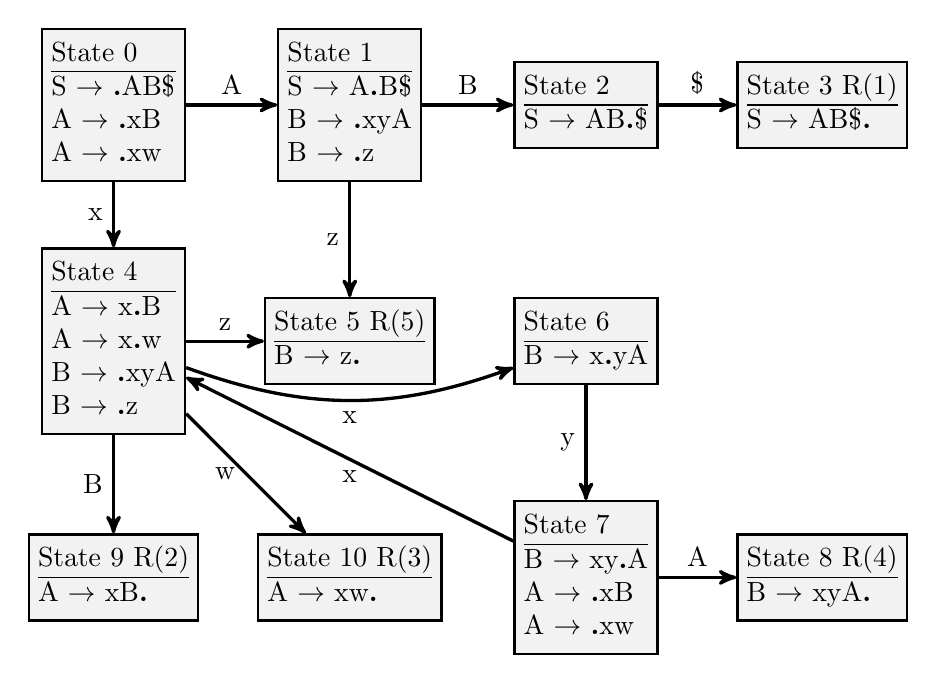
\begin{tikzpicture}
    \node[state, shape=rectangle] (0) {
    \makecell[l] {
    State 0 \\
    \hline
    S $\rightarrow$ \textbf{.}AB\$ \\
    A $\rightarrow$ \textbf{.}xB \\
    A $\rightarrow$ \textbf{.}xw
    }};
    \node[state, shape=rectangle, right of=0] (1) {
    \makecell[l] {
    State 1 \\
    \hline
    S $\rightarrow$ A\textbf{.}B\$ \\
    B $\rightarrow$ \textbf{.}xyA \\
    B $\rightarrow$ \textbf{.}z
    }};
    \node[state, shape=rectangle, right of=1] (2) {
    \makecell[l] {
    State 2 \\
    \hline
    S $\rightarrow$ AB\textbf{.}\$
    }};
    \node[state, shape=rectangle, right of=2] (3) {
    \makecell[l] {
    State 3 R(1)\\
    \hline
    S $\rightarrow$ AB\$\textbf{.} \\
    }};
    \node[state, shape=rectangle, below of=0] (4) {
    \makecell[l] {
    State 4\\
    \hline
    A $\rightarrow$ x\textbf{.}B \\
    A $\rightarrow$ x\textbf{.}w \\
    B $\rightarrow$ \textbf{.}xyA \\
    B $\rightarrow$ \textbf{.}z
    }};
    \node[state, shape=rectangle, below of=1] (5) {
    \makecell[l] {
    State 5 R(5)\\
    \hline
    B $\rightarrow$ z\textbf{.} \\
    }};
    \node[state, shape=rectangle, below of=2] (6) {
    \makecell[l] {
    State 6 \\
    \hline
    B $\rightarrow$ x\textbf{.}yA \\
    }};
    \node[state, shape=rectangle, below of=6] (7) {
    \makecell[l] {
    State 7 \\
    \hline
    B $\rightarrow$ xy\textbf{.}A \\
    A $\rightarrow$ \textbf{.}xB \\
    A $\rightarrow$ \textbf{.}xw
    }};
    \node[state, shape=rectangle, right of=7] (8) {
    \makecell[l] {
    State 8 R(4)\\
    \hline
    B $\rightarrow$ xyA\textbf{.} \\
    }};
    \node[state, shape=rectangle, below of=4] (9) {
    \makecell[l] {
    State 9 R(2)\\
    \hline
    A $\rightarrow$ xB\textbf{.} \\
    }};
    \node[state, shape=rectangle, below of=5] (10) {
    \makecell[l] {
    State 10 R(3)\\
    \hline
    A $\rightarrow$ xw\textbf{.} \\
    }};
    \draw[very thick]
          (0) edge[right, above] node{A} (1)
          (0) edge[right, left] node{x} (4)
          (1) edge[right, above] node{B} (2)
          (1) edge[right, left] node{z} (5)
          (2) edge[right, above] node{\$} (3)
          (4) edge[right, above] node{z} (5)
          (4) edge[bend right=20, below] node{x} (6)
          (6) edge[left, left] node{y} (7)
          (7) edge[left, below] node{x} (4)
          (7) edge[left, above] node{A} (8)
          (4) edge[left, left] node{B} (9)
          (4) edge[left, left] node{w} (10);
  \end{tikzpicture}
\end{multicols}
\subsubsection{GoTo/Action Table}
\noindent
  \begin{tabular}{|c|c|c|c|c|c|c|c|c|c|c|}
    \hline
	  & \multicolumn{8}{c|}{\textbf{Symbol}} & \\
    \hline
	  & \thead{x} & \thead{w} & \thead{y} & \thead{z} & \thead{A} & \thead{\$} & \thead{B} & \thead{S}  & \thead{Action}\\
    \hline
	\textbf{0}  & 4 &    &   &   & 1 &   &   &   & Shift \\
    \hline
	\textbf{1}  &   &    &   &   &   &   & 2 &   & Shift \\
    \hline
	\textbf{2}  &   &    &   &   &   & 3 &   &   & Shift \\
    \hline
	\textbf{3}  &   &    &   &   &   &   &   &   & Accept R(1) \\
    \hline
	\textbf{4}  &   & 10 &   & 5 &   &   & 9 &   & Shift \\
    \hline
	\textbf{5}  &   &    &   &   &   &   &   &   & Reduce 5 \\
    \hline
	\textbf{6}  &   &    & 7 &   &   &   &   &   & Shift \\
    \hline
	\textbf{7}  & 4 &    &   &   & 8 &   &   &   & Shift \\
    \hline
	\textbf{8}  &   &    &   &   &   &   &   &   & Reduce 4 \\
    \hline
	\textbf{9}  &   &    &   &   &   &   &   &   & Reduce 2 \\
    \hline
	\textbf{10} &   &    &   &   &   &   &   &   & Reduce 3 \\
    \hline
  \end{tabular}

\newpage
\renewcommand\thechapter{Q3}
\chapter{Take Home Quiz 3}
\begin{multicols}{2}
  \begin{enumerate}
    \setlength\itemsep{-.25em}
    \item S $\rightarrow$ E\$
    \item E $\rightarrow$ E+T
    \item E $\rightarrow$ T
    \item T $\rightarrow$ ID
    \item T $\rightarrow$ (E)
     \newline\newline\newline\newline\newline\newline\newline\newline\newline\newline\newline\newline\newline\newline\newline\newline\newline\newline\newline\newline\newline\newline
  \end{enumerate}
  \vspace{-50pt}
  \setlength{\leftskip}{-15em}
  \subsubsection{State Diagram}
  \vspace{-10pt}
  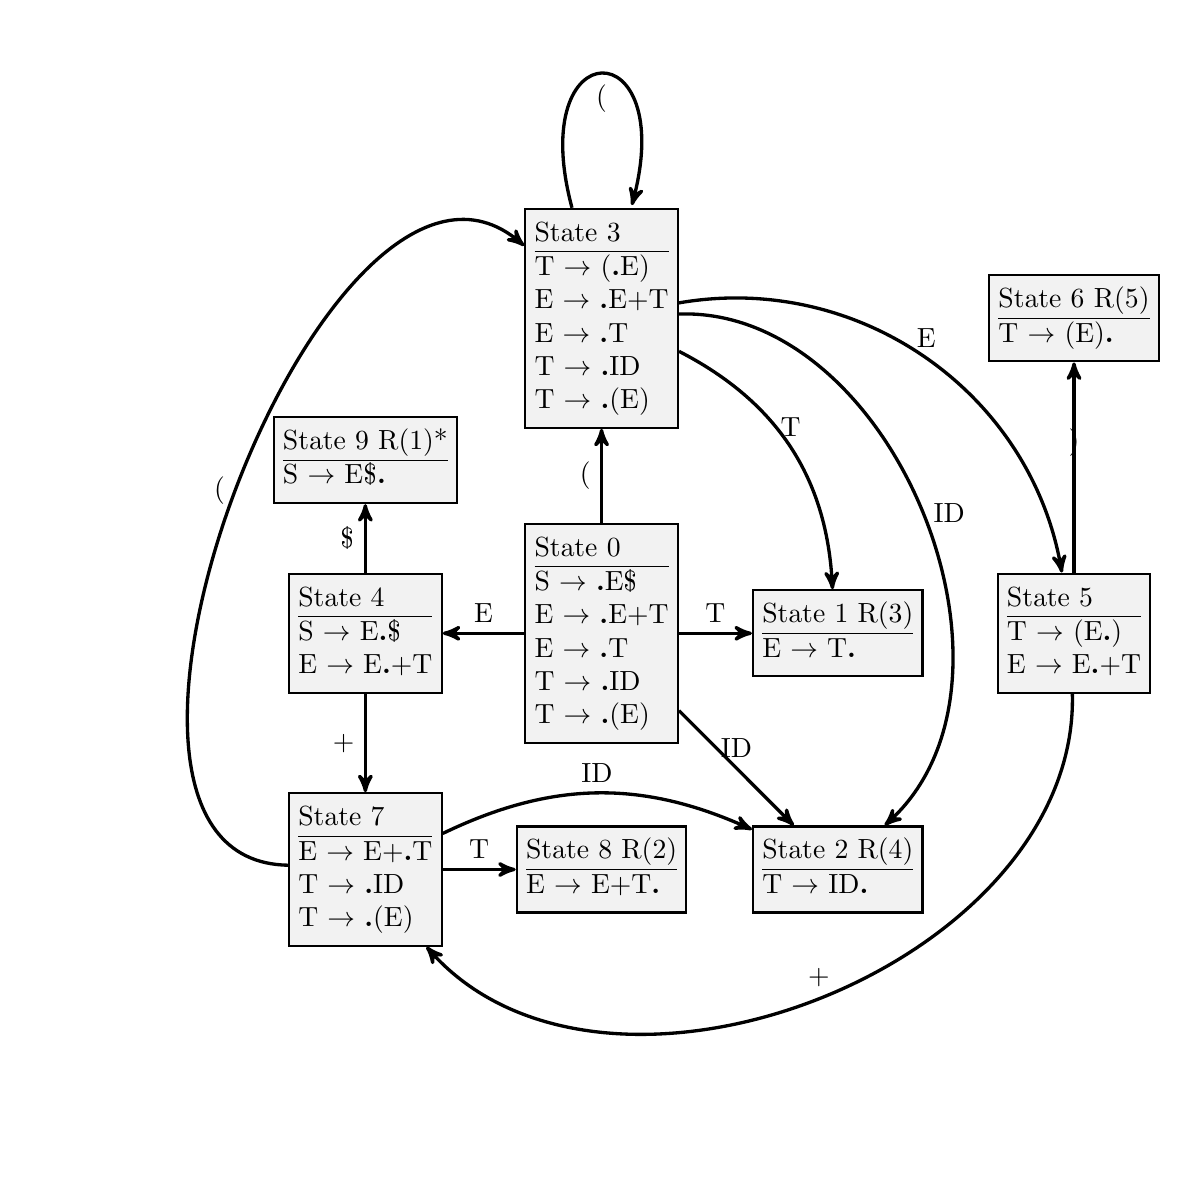
\begin{tikzpicture}
    \node[state, shape=rectangle] (0) {
    \makecell[l] {
    State 0 \\
    \hline
    S $\rightarrow$ \textbf{.}E\$ \\
    E $\rightarrow$ \textbf{.}E+T \\
    E $\rightarrow$ \textbf{.}T \\
    T $\rightarrow$ \textbf{.}ID \\
    T $\rightarrow$ \textbf{.}(E)
    }};
    \node[state, shape=rectangle, right of=0] (1) {
    \makecell[l] {
    State 1 R(3)\\
    \hline
    E $\rightarrow$ T\textbf{.}
    }};
    \node[state, shape=rectangle, below of=0, right of=0] (2) {
    \makecell[l] {
    State 2 R(4)\\
    \hline
    T $\rightarrow$ ID\textbf{.}
    }};
    \node[state, shape=rectangle, above of=0, yshift=10mm] (3) {
    \makecell[l] {
    State 3 \\
    \hline
    T $\rightarrow$ (\textbf{.}E) \\
    E $\rightarrow$ \textbf{.}E+T \\
    E $\rightarrow$ \textbf{.}T \\
    T $\rightarrow$ \textbf{.}ID \\
    T $\rightarrow$ \textbf{.}(E)
    }};
    \node[state, shape=rectangle, left of=0] (4) {
    \makecell[l] {
    State 4\\
    \hline
    S $\rightarrow$ E\textbf{.}\$ \\
    E $\rightarrow$ E\textbf{.}+T
    }};
    \node[state, shape=rectangle, right of=1] (5) {
    \makecell[l] {
    State 5\\
    \hline
    T $\rightarrow$ (E\textbf{.}) \\
    E $\rightarrow$ E\textbf{.}+T
    }};
    \node[state, shape=rectangle, above of=5, yshift=10mm] (6) {
    \makecell[l] {
    State 6 R(5)\\
    \hline
    T $\rightarrow$ (E)\textbf{.}
    }};
    \node[state, shape=rectangle, below of=4] (7) {
    \makecell[l] {
    State 7\\
    \hline
    E $\rightarrow$ E+\textbf{.}T \\
    T $\rightarrow$ \textbf{.}ID \\
    T $\rightarrow$ \textbf{.}(E)
    }};
    \node[state, shape=rectangle, below of=0] (8) {
    \makecell[l] {
    State 8 R(2)\\
    \hline
    E $\rightarrow$ E+T\textbf{.}
    }};
    \node[state, shape=rectangle, above of=4, yshift=-8mm] (9) {
    \makecell[l] {
    State 9 R(1)*\\
    \hline
    S $\rightarrow$ E\$\textbf{.} \\
    }};
    \draw[very thick]
          (0) edge[right, above] node{T} (1)
          (0) edge[left, above] node{ID} (2)
          (0) edge[right, left] node{(} (3)
          (0) edge[right, above] node{E} (4)
          (3) edge[bend left=30, above] node{T} (1)
          (3) edge[bend left=70, right] node{ID} (2)
          (3) edge[loop above, below] node{(} (3)
          (3) edge[bend left=45, above] node{E} (5)
          (4) edge[right, left] node{+} (7)
          (4) edge[right, left] node{\$} (9)
          (5) edge[right, above] node{)} (6)
          (5) edge[bend left=70, above] node{+} (7)
          (7) edge[bend left=25, above] node{ID} (2)
          (7) edge[bend left=110, left] node{(} (3)
          (7) edge[right, above] node{T} (8);
  \end{tikzpicture}
\end{multicols}
\vspace{-40pt}
\subsubsection{GoTo/Action Table}
\noindent
  \begin{tabular}{|c|c|c|c|c|c|c|c|c|c|c|}
    \hline
	  & \multicolumn{8}{c|}{\textbf{Symbol}} & \\
    \hline
	  & \thead{+} & \thead{ID} & \thead{(} & \thead{)} & \thead{T} & \thead{E} & \thead{\$} & \thead{S}  & \thead{Action}\\
    \hline
	\textbf{0} &   & 2 & 3 &   & 1 & 4 &   &   & Shift \\
    \hline
	\textbf{1} &   &   &   &   &   &   &   &   & Reduce 3 \\
    \hline
	\textbf{2} &   &   &   &   &   &   &   &   & Reduce 4 \\
    \hline
	\textbf{3} &   & 2 & 3 &   & 1 & 5 &   &   & Shift \\
    \hline
	\textbf{4} & 7 &   &   &   &   &   & 9 &   & Shift \\
    \hline
	\textbf{5} & 7 &   &   & 6 &   &   &   &   & Shift \\
    \hline
	\textbf{6} &   &   &   &   &   &   &   &   & Reduce 5 \\
    \hline
	\textbf{7} &   & 2 & 3 &   & 8 &   &   &   & Shift \\
    \hline
	\textbf{8} &   &   &   &   &   &   &   &   & Reduce 2 \\
    \hline
	\textbf{9} &   &   &   &   &   &   &   &   & Accept R(1) \\
    \hline
  \end{tabular}

\renewcommand\thechapter{E1}
\chapter{Midterm Exam - Practice Questions}
\section{Q1:}
\begin{enumerate}[label=(\alph*)]
  \item Give regular expressions for the following languages. The alphabets are given at the end.
  \begin{enumerate}[label=\roman*.]
    \item Contains exactly one a. \{a, b\} \hspace{1em} \textbf{b*ab*}
    
    \item Has 00 or 11 as a substring. \{0, 1\} \textbf{(011)*(00|11)(011)*} (professor) or \textbf{0*1*(00|11)0*1*} (mine)
  \end{enumerate}
  \item Describe the following in English.
  \begin{enumerate}[label=\roman*.]
    \item (a|b)* : \hspace{3.3em} \textbf{Strings made up of zero or more a's or b's, including the empty string}
    \item (a|b)*ab(a|b)* : \textbf{Strings containing ab as a substring}
  \end{enumerate}
  \item Draw the NFA for (b) (ii).
  
  \subsubsection{Thompson's Construction Algorithm - Professor Answer}
  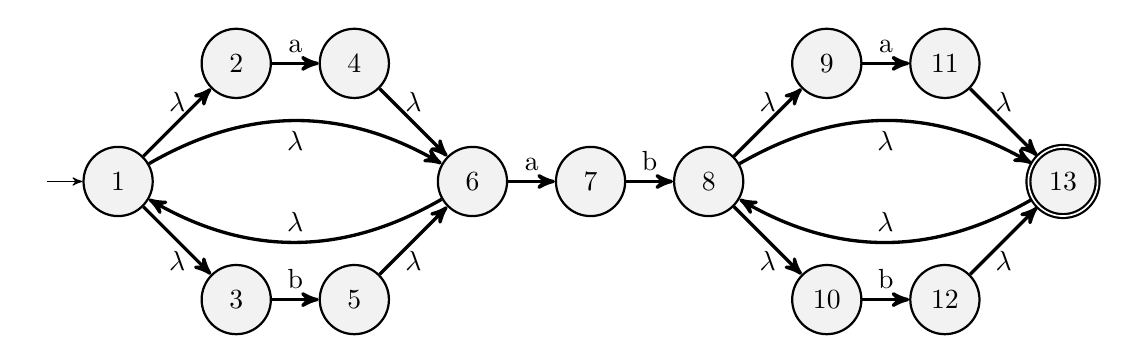
\begin{tikzpicture}[node distance=1.5cm]
    \node[state, initial] (1) {$1$};
    \node[state, above of=1, right of=1] (2) {$2$};
    \node[state, below of=1, right of=1] (3) {$3$};
    \node[state, right of=2] (4) {$4$};
    \node[state, right of=3] (5) {$5$};
    \node[state, below of=4, right of=4] (6) {$6$};
    \node[state, right of=6] (7) {$7$};
    \node[state, right of=7] (8) {$8$};
    \node[state, above of=8, right of=8] (9) {$9$};
    \node[state, below of=8, right of=8] (10) {$10$};
    \node[state, right of=9] (11) {$11$};
    \node[state, right of=10] (12) {$12$};
    \node[state, accepting, below of=11, right of=11] (13) {$13$};
    \draw[very thick]
      (1) edge[left, above] node{$\lambda$} (2)
      (1) edge[left, below] node{$\lambda$} (3)
      (1) edge[bend left, below] node{$\lambda$} (6)
      (2) edge[left, above] node{a} (4)
      (3) edge[left, above] node{b} (5)
      (4) edge[left, above] node{$\lambda$} (6)
      (5) edge[left, below] node{$\lambda$} (6)
      (6) edge[bend left, above] node{$\lambda$} (1)
      (6) edge[left, above] node{a} (7)
      (7) edge[left, above] node{b} (8)
      (8) edge[left, above] node{$\lambda$} (9)
      (8) edge[left, below] node{$\lambda$} (10)
      (8) edge[bend left, below] node{$\lambda$} (13)
      (9) edge[left, above] node{a} (11)
      (10) edge[left, above] node{b} (12)
      (11) edge[left, above] node{$\lambda$} (13)
      (12) edge[left, below] node{$\lambda$} (13)
      (13) edge[bend left, above] node{$\lambda$} (8);
  \end{tikzpicture}
  
  \subsubsection{Generic NFA - My Answer}
  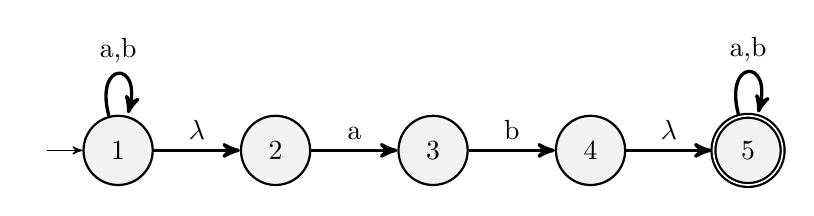
\begin{tikzpicture}[node distance=2cm]
    \node[state, initial] (1) {$1$};
    \node[state, right of=1] (2) {$2$};
    \node[state, right of=2] (3) {$3$};
    \node[state, right of=3] (4) {$4$};
    \node[state, accepting, right of=4] (5) {$5$};
    \draw[very thick]
      (1) edge[loop above] node{a,b} (1)
      (1) edge[left, above] node{$\lambda$} (2)
      (2) edge[left, above] node{a} (3)
      (3) edge[left, above] node{b} (4)
      (4) edge[left, above] node{$\lambda$} (5)
      (5) edge[loop above] node{a,b} (5);
  \end{tikzpicture}
  
  
  \item Consider the following NFA and complete the corresponding DFA (transition table) below.\newline
\vspace{-1.5em}
\begin{multicols}{2}
  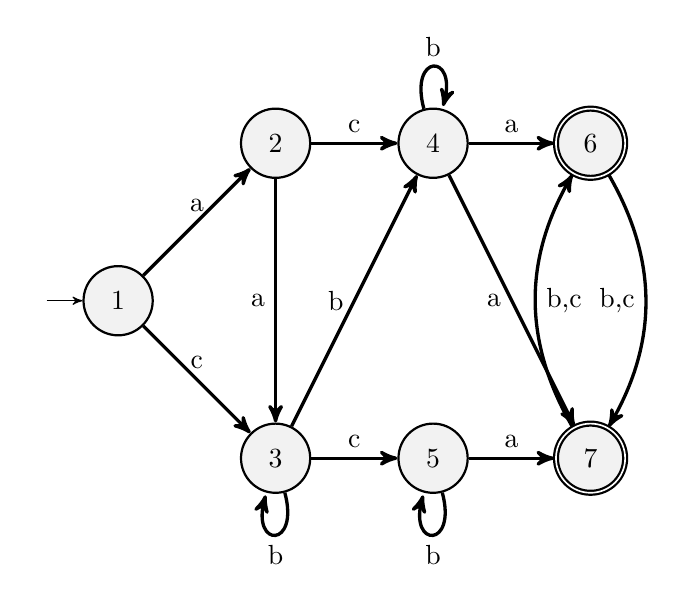
\begin{tikzpicture}[node distance=2cm]
    \node[state, initial] (1) {$1$};
    \node[state, above of=1, right of=1] (2) {$2$};
    \node[state, below of=1, right of=1] (3) {$3$};
    \node[state, right of=2] (4) {$4$};
    \node[state, right of=3] (5) {$5$};
    \node[state, accepting, right of=4] (6) {$6$};
    \node[state, accepting, right of=5] (7) {$7$};
    \draw[very thick]
      (1) edge[left, above] node{a} (2)
      (1) edge[left, above] node{c} (3)
      (2) edge[left, left] node{a} (3)
      (2) edge[left, above] node{c} (4)
      (3) edge[loop below] node{b} (3)
      (3) edge[left, left] node{b} (4)
      (3) edge[left, above] node{c} (5)
      (4) edge[loop above] node{b} (4)
      (4) edge[left, above] node{a} (6)
      (4) edge[left, left] node{a} (7)
      (5) edge[loop below] node{b} (5)
      (5) edge[left, above] node{a} (7)
      (6) edge[bend left, left] node{b,c} (7)
      (7) edge[bend left, right] node{b,c} (6);
  \end{tikzpicture}
  \newline\newline\newline\newline
  \begin{tabular}{|c|c|c|c|c|}
    \hline
	  \thead{State} & \thead{a} & \thead{b} & \thead{c} & \thead{Final}\\
    \hline
	\textbf{1}   & \{2\}       & \textemdash & \{3\}       & No \\
    \hline
	\textbf{2}   & \{3\}       & \textemdash & \{4\}       & No \\
    \hline
	\textbf{3}   & \textemdash & \{3,4\}     & \{5\}       & No \\
    \hline
	\textbf{4}   & \{6,7\}     & \{4\}       & \textemdash & No \\
    \hline
	\textbf{3,4} & \{6,7\}     & \{3,4\}     & \textemdash & No \\
    \hline
	\textbf{5}   & \{7\}       & \{5\}       & \textemdash & No \\
    \hline
	\textbf{6,7} & \textemdash & \{6,7\}     & \{6,7\}     & Yes \\
    \hline
	\textbf{7}   & \textemdash & \{6\}       & \{6\}       & Yes \\
    \hline
	\textbf{6}   & \textemdash & \{7\}       & \{7\}       & Yes \\
    \hline
  \end{tabular}
\end{multicols}
\end{enumerate}

\newpage
\section{Q2:}
\noindent Consider the following grammar.
\begin{enumerate}
  \item S $\rightarrow$ AB\$
  \item A $\rightarrow$ xAz
  \item A $\rightarrow$ yAz
  \item A $\rightarrow$ $\lambda$
  \item B $\rightarrow$ Bz
  \item B $\rightarrow$ $\lambda$
  \begin{enumerate}
    \item What are the terminals and the non-terminals?\newline
    \textbf{terminals:} \{x, y, z, \$\}\newline
    \textbf{non-terminals:} \{S, A, B\}\newline
    \item Derive xyzzz\$ using LMD.
    \vspace{-1em}
    \begin{multicols}{2}
      \begin{itemize}
        \setlength\itemsep{-.25em}
        \item[] S $\rightarrow$ AB\$
        \item[] \hspace{.9em}$\rightarrow$ xAzB\$
        \item[] \hspace{.9em}$\rightarrow$ xyAzzB\$
        \item[] \hspace{.9em}$\rightarrow$ xyzzB\$
        \item[] \hspace{.9em}$\rightarrow$ xyzzBz\$
        \item[] \hspace{.9em}$\rightarrow$ xyzzz\$
      \end{itemize}
      \begin{itemize}
        \setlength\itemsep{-.25em}
        \item[] Rule 1
        \item[] Rule 2
        \item[] Rule 3
        \item[] Rule 4
        \item[] Rule 5
        \item[] Rule 6
      \end{itemize}
    \end{multicols}
    \item Draw the parse tree for the above string.\newline
    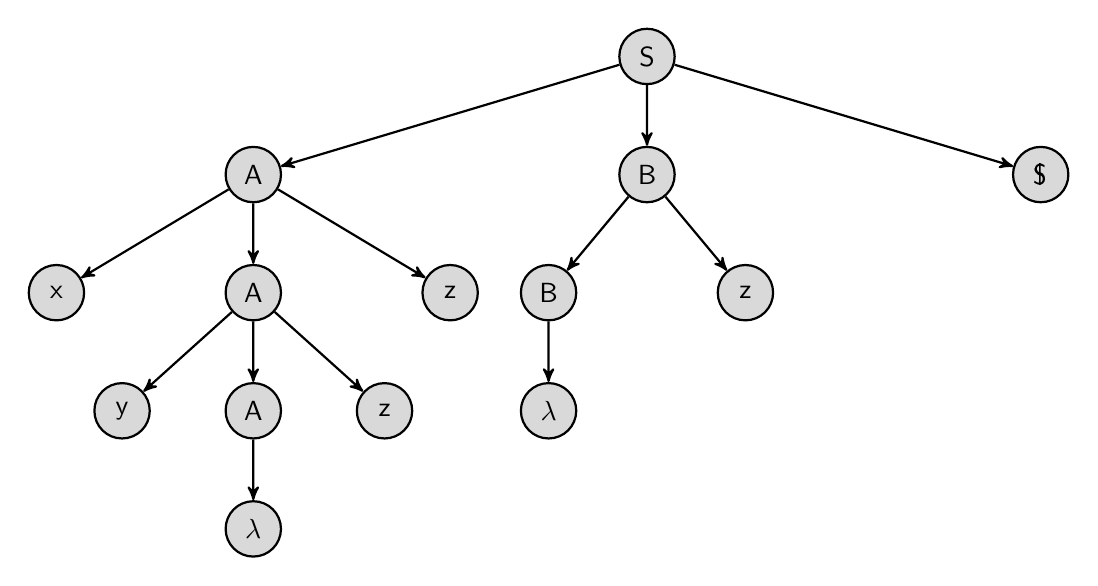
\begin{tikzpicture}[font=\sffamily,thick,level/.style={sibling distance=50mm/#1}]
    \node[vertex]
    {S}
        child {
            node[vertex] {A}
            child { node[vertex] {x} }
            child {
                node[vertex] {A}
                child { node[vertex] {y} }
                child {
                    node[vertex] {A}
                    child { node[vertex] {$\lambda$} }
                }
                child { node[vertex] {z} }
            }
            child { node[vertex] {z} }
        } child {
            node[vertex] {B}
            child {
                node[vertex] {B}
                child { node[vertex] {$\lambda$} }
            }
            child { node[vertex] {z} }
        } child { node[vertex] {\$} }
    ;
\end{tikzpicture}
    \item Describe the strings generated by this grammar.\newline
    \textbf{Strings of the form $(x|y)^i$$z^j$ where $a^k$ represents \textit{k} occurrences of symbol \textit{a}, \& \textit{i $\le$ j}}\newline(professor)\newline
    
    \textbf{All strings that starting with zero or more x's ending with a z for ever x, followed by zero or more y's ending with a z for every y, and ending in zero or more z's, including the empty string.} (mine)
\newpage
    \item Given the following grammar, fill in the blanks below. Is this LL(1)? Why or why not?
    \begin{multicols}{2}
      \begin{enumerate}[label=\arabic*.]
        \item S $\rightarrow$ A\$
        \item A $\rightarrow$ (AB)
        \item A $\rightarrow$ $\lambda$
        \item B $\rightarrow$ (A)
        \item B $\rightarrow$ x\newline
      \end{enumerate}
\setlength{\leftskip}{-12em}
      \textbf{First Sets}\newline
      First (B) = First((A)) $\cup$ First(x) =\textbf{\{(, x\} $\leftarrow$ Final set of B}\newline
      First (A) = First((AB)) $\cup$ First($\lambda$) = \textbf{\{(, $\lambda$\} $\leftarrow$ Final set of A}\newline
      First (S) = First(A\$)\newline
      \indent\hspace{1.5cm}= (First(A) - $\lambda$) $\cup$ First(\$) = \textbf{\{(, \$\} $\leftarrow$ Final set of S}\newline
    \end{multicols}
    \vspace{-1em}
    \textbf{Follow Sets}\newline
    Follow (B) = First()) = \textbf{ \{)\} $\leftarrow$ Final set of B}\newline
    Follow (A) = First(\$) $\cup$ First(B) $\cup$ First())\newline
    \indent\hspace{1.75cm}= \{\$\} $\cup$ First(B) $\cup$ \{)\}\newline
    \indent\hspace{1.75cm}= \textbf{ \{\$, x, (, )\} $\leftarrow$ Final set of A}\newline
    Follow (S) = First(\$) = \textbf{ \{\} $\leftarrow$ Final set of S}\newline

    \textbf{Predict Sets}\newline
    predict (1. S $\rightarrow$ A\$) = First(A\$) = (First(A) - $\lambda$) $\cup$ \{\$\}= \textbf{ \{(, \$\} $\leftarrow$ Final}\newline
    predict (2. A $\rightarrow$ (AB)) = \textbf{ \{(\} $\leftarrow$ Final} \hspace{2em} note: just A $\rightarrow$ (\newline
    predict (3. A $\rightarrow$ $\lambda$) = (First(RHS) - $\lambda$) $\cup$ Follow(A) = \textbf{ \{\$, x, (, )\} $\leftarrow$ Final}\newline
    predict (4. B $\rightarrow$ (A)) = \textbf{ \{(\} $\leftarrow$ Final}\newline
    predict (5. B $\rightarrow$ x) = \textbf{ \{x\} $\leftarrow$ Final}\newline
    
     
    \begin{multicols}{2}
      \textbf{First and Follow Sets}\newline
      \begin{tabular}{|c|c|c|}
        \hline
        \thead{Sybmol} & \thead{First Set} & \thead{Follow Set} \\
        \hline
        \textbf{S} & \{(, \$\}     & \{\} \\
        \hline
        \textbf{A} & \{(, $\lambda$\}     & \{x, (, ), \$\} \\
        \hline
        \textbf{B} & \{x, (\}  & \{)\} \\
        \hline
      \end{tabular} \newline
      \textbf{LL(1) Parse Table}\newline
      \begin{tabular}{|c|c|c|c|c|}
        \hline
        \thead{Sybmol} & \thead{x} & \thead{(} & \thead{)} & \thead{\$}  \\
        \hline
        \textbf{S} & err & 1   & err & 1 \\
        \hline
        \textbf{A} & 3   & 2,3 & 3   & 3 \\
        \hline
        \textbf{B} & 5   & 4   &     & \\
        \hline
      \end{tabular}
    \end{multicols}
    \textbf{No, NOT LL(1)}, because of ambiguity on (. Cannot reduce A because of predict 2,3
  \end{enumerate}
\end{enumerate}
\newpage
\section{Q3:}
\noindent Complete the CFSM for the following grammar. It is LR(0)?
\begin{multicols}{2}
\begin{enumerate}
  \item S $\rightarrow$ A\$
  \item A $\rightarrow$ xBx
  \item A $\rightarrow$ xyBx
  \item B $\rightarrow$ Bz
  \item B $\rightarrow$ z\newline\newline\newline\newline\newline\newline\newline\newline\newline\newline\newline\newline
  \end{enumerate}
  \setlength{\leftskip}{-10em}
  \subsubsection{State Diagram}
  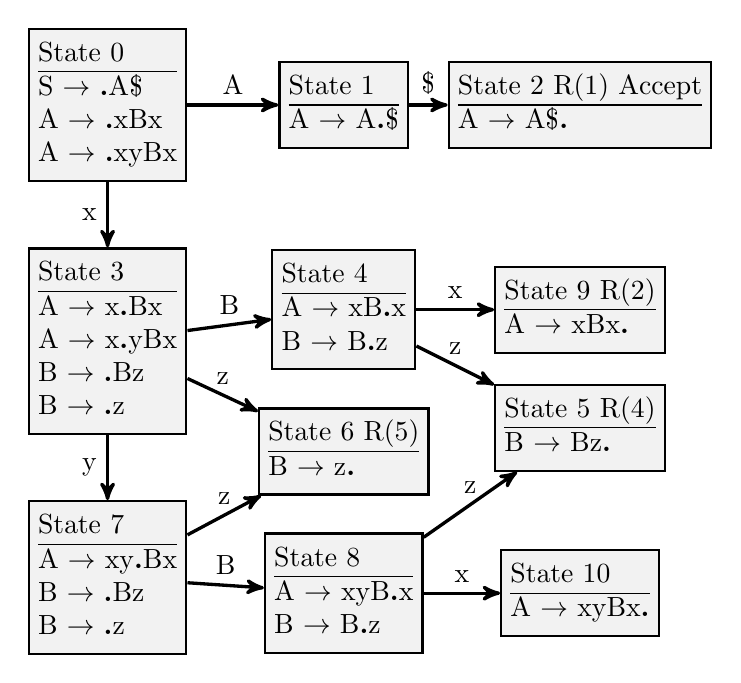
\begin{tikzpicture}
    \node[state, shape=rectangle] (0) {
    \makecell[l] {
    State 0 \\
    \hline
    S $\rightarrow$ \textbf{.}A\$ \\
    A $\rightarrow$ \textbf{.}xBx \\
    A $\rightarrow$ \textbf{.}xyBx
    }};
    \node[state, shape=rectangle, right of=0] (1) {
    \makecell[l] {
    State 1 \\
    \hline
    A $\rightarrow$ A\textbf{.}\$
    }};
    \node[state, shape=rectangle, right of=1] (2) {
    \makecell[l] {
    State 2 R(1) Accept\\
    \hline
    A $\rightarrow$ A\$\textbf{.}
    }};
    \node[state, shape=rectangle, below of=0] (3) {
    \makecell[l] {
    State 3 \\
    \hline
    A $\rightarrow$ x\textbf{.}Bx \\
    A $\rightarrow$ x\textbf{.}yBx \\
    B $\rightarrow$ \textbf{.}Bz \\
    B $\rightarrow$ \textbf{.}z
    }};
    \node[state, shape=rectangle, below of=1, yshift=4mm] (4) {
    \makecell[l] {
    State 4 \\
    \hline
    A $\rightarrow$ xB\textbf{.}x \\
    B $\rightarrow$ B\textbf{.}z \\
    }};
    \node[state, shape=rectangle, below of=2, yshift=4mm] (9) {
    \makecell[l] {
    State 9 R(2) \\
    \hline
    A $\rightarrow$ xBx\textbf{.} \\
    }};
    \node[state, shape=rectangle, below of=9, yshift=15mm] (5) {
    \makecell[l] {
    State 5 R(4)\\
    \hline
    B $\rightarrow$ Bz\textbf{.}
    }};
    \node[state, shape=rectangle, below of=4, yshift=12mm] (6) {
    \makecell[l] {
    State 6 R(5) \\
    \hline
    B $\rightarrow$ z\textbf{.}
    }};
    \node[state, shape=rectangle, below of=3] (7) {
    \makecell[l] {
    State 7 \\
    \hline
    A $\rightarrow$ xy\textbf{.}Bx \\
    B $\rightarrow$ \textbf{.}Bz \\
    B $\rightarrow$ \textbf{.}z
    }};
    \node[state, shape=rectangle, below of=6, yshift=12mm] (8) {
    \makecell[l] {
    State 8 \\
    \hline
    A $\rightarrow$ xyB\textbf{.}x \\
    B $\rightarrow$ B\textbf{.}z \\
    }};
    \node[state, shape=rectangle, right of=8] (10) {
    \makecell[l] {
    State 10 \\
    \hline
    A $\rightarrow$ xyBx\textbf{.}
    }};
    \draw[very thick]
          (0) edge[right, above] node{A} (1)
          (0) edge[right, left] node{x} (3)
          (1) edge[right, above] node{\$} (2)
          (3) edge[right, above] node{B} (4)
          (3) edge[right, above] node{z} (6)
          (3) edge[right, left] node{y} (7)
          (4) edge[right, above] node{x} (9)
          (4) edge[right, above] node{z} (5)
          (7) edge[right, above] node{z} (6)
          (7) edge[right, above] node{B} (8)
          (8) edge[right, above] node{z} (5)
          (8) edge[right, above] node{x} (10);
  \end{tikzpicture}
\end{multicols}
\textbf{Yes, LR(0)}, because the grammar has no conflicts on the CFSM; no shift reduce (S/R) conflicts or reduce reduce (R/R) conflicts
\begin{multicols}{2}
      \begin{enumerate}[label=\arabic*.]
        \item S $\rightarrow$ A\$
        \item A $\rightarrow$ xBx
        \item A $\rightarrow$ xyBx
        \item B $\rightarrow$ Bz
        \item B $\rightarrow$ z
      \end{enumerate}
\setlength{\leftskip}{-12em}
      \textbf{First Sets}\newline
      First (B) = \textbf{\{z\} $\leftarrow$ Final set of B}\newline
      First (A) = \textbf{\{x\} $\leftarrow$ Final set of A}\newline
      First (S) = \textbf{\{x\} $\leftarrow$ Final set of S}\newline
\end{multicols}
\begin{multicols}{2}
\noindent\textbf{Follow Sets}\newline
    Follow (B) = \textbf{ \{x, z\} $\leftarrow$ Final set of B}\newline
    Follow (A) = \textbf{ \{\$\} $\leftarrow$ Final set of A}\newline
    Follow (S) =  \textbf{ \{\} $\leftarrow$ Final set of S}\newline\newline\newline

\noindent\textbf{Predict Sets}\newline
    predict (1. S $\rightarrow$ A\$) = \textbf{ \{x\} $\leftarrow$ Final}\newline
    predict (2. A $\rightarrow$ xBx) = \textbf{ \{x\} $\leftarrow$ Final}\newline
    predict (3. A $\rightarrow$ xyBx) = \textbf{ \{x\} $\leftarrow$ Final}\newline
    predict (4. B $\rightarrow$ Bz) = \textbf{ \{z\} $\leftarrow$ Final}\newline
    predict (5. B $\rightarrow$ z) = \textbf{ \{z\} $\leftarrow$ Final}\newline
\end{multicols}

\renewcommand\thechapter{X1}
\chapter{Midterm Examples - First, Follow, Predict sets}
\section{Quiz 6: In Class}
\vspace{-1em}
\begin{multicols}{2}
      \begin{enumerate}[label=\arabic*.]
        \item S $\rightarrow$ AB\$
        \item A $\rightarrow$ xB
        \item A $\rightarrow$ xw
        \item B $\rightarrow$ xyA
        \item B $\rightarrow$ z
      \end{enumerate}
\setlength{\leftskip}{-12em}
      \textbf{First Sets}\newline
      First (B) = \textbf{\{x\} $\leftarrow$ Final set of B}\newline
      First (A) = \textbf{\{x\} $\leftarrow$ Final set of A}\newline
      First (S) = \textbf{\{x, z\} $\leftarrow$ Final set of S}\newline
\end{multicols}
\begin{multicols}{2}
\noindent\textbf{Follow Sets}\newline
    Follow (B) = \textbf{ \{x, z, \$\} $\leftarrow$ Final set of B}\newline
    Follow (A) = \textbf{ \{x, z, \$\} $\leftarrow$ Final set of A}\newline
    Follow (S) =  \textbf{ \{\} $\leftarrow$ Final set of S}\newline\newline\newline

\noindent\textbf{Predict Sets}\newline
    predict (1. S $\rightarrow$ AB\$) = \textbf{ \{x\} $\leftarrow$ Final}\newline
    predict (2. A $\rightarrow$ xB) = \textbf{ \{x\} $\leftarrow$ Final}\newline
    predict (3. A $\rightarrow$ xw) = \textbf{ \{x\} $\leftarrow$ Final}\newline
    predict (4. B $\rightarrow$ xyA) = \textbf{ \{x\} $\leftarrow$ Final}\newline
    predict (5. B $\rightarrow$ z) = \textbf{ \{z\} $\leftarrow$ Final}\newline
\end{multicols}

\section{Quiz 3: Take home}
\vspace{-1em}
\begin{multicols}{2}
      \begin{enumerate}[label=\arabic*.]
        \item S $\rightarrow$ E\$
        \item E $\rightarrow$ E + T
        \item E $\rightarrow$ T
        \item T $\rightarrow$ ID
        \item T $\rightarrow$ (E)
      \end{enumerate}
\setlength{\leftskip}{-12em}
      \textbf{First Sets}\newline
      First (T) = \textbf{\{ID, (\} $\leftarrow$ Final set of T}\newline
      First (E) = \textbf{\{ID, (\} $\leftarrow$ Final set of E}\newline
      First (S) = \textbf{\{ID, (\} $\leftarrow$ Final set of S}\newline
\end{multicols}
\begin{multicols}{2}
\noindent\textbf{Follow Sets}\newline
    Follow (T) = \textbf{ \{+, ), \$\} $\leftarrow$ Final set of T}\newline
    Follow (E) = \textbf{ \{+, ), \$\} $\leftarrow$ Final set of E}\newline
    Follow (S) =  \textbf{ \{\} $\leftarrow$ Final set of S}\newline\newline\newline

\noindent\textbf{Predict Sets}\newline
    predict (1. S $\rightarrow$ E\$ = \textbf{ \{(, ID\} $\leftarrow$ Final}\newline
    predict (2. E $\rightarrow$ E + T = \textbf{ \{(, ID\} $\leftarrow$ Final}\newline
    predict (3. E $\rightarrow$ T = \textbf{ \{(, ID\} $\leftarrow$ Final}\newline
    predict (4. T $\rightarrow$ ID = \textbf{ \{ID\} $\leftarrow$ Final}\newline
    predict (5. T $\rightarrow$ (E) = \textbf{ \{(\} $\leftarrow$ Final}\newline
\end{multicols}


\section{Q2: Practice Exam 1}
\vspace{-1em}
\begin{multicols}{2}
      \begin{enumerate}[label=\arabic*.]
        \item S $\rightarrow$ AB\$
        \item A $\rightarrow$ xAz
        \item A $\rightarrow$ yAz
        \item A $\rightarrow$ $\lambda$
        \item B $\rightarrow$ Bz
        \item B $\rightarrow$ $\lambda$
      \end{enumerate}
\setlength{\leftskip}{-12em}
      \textbf{First Sets}\newline
      First (B) = \textbf{\{z, $\lambda$\} $\leftarrow$ Final set of B}\newline
      First (A) = \textbf{\{x, y, $\lambda$\} $\leftarrow$ Final set of A}\newline
      First (S) = \textbf{\{x, y, z, \$\} $\leftarrow$ Final set of S}\newline
\end{multicols}
\begin{multicols}{2}
\noindent\textbf{Follow Sets}\newline
    Follow (B) = \textbf{ \{z, \$\} $\leftarrow$ Final set of B}\newline
    Follow (A) = \textbf{ \{z, \$\} $\leftarrow$ Final set of A}\newline
    Follow (S) =  \textbf{ \{\} $\leftarrow$ Final set of S}\newline\newline\newline\newline

\noindent\textbf{Predict Sets}\newline
    predict (1. S $\rightarrow$ AB\$) = \textbf{ \{x, y, z, \$\} $\leftarrow$ Final}\newline
    predict (2. A $\rightarrow$ xAz) = \textbf{ \{x\} $\leftarrow$ Final}\newline
    predict (3. A $\rightarrow$ yAz) = \textbf{ \{y\} $\leftarrow$ Final}\newline
    predict (4. A $\rightarrow$ $\lambda$) = \textbf{ \{z, \$\} $\leftarrow$ Final}\newline
    predict (5. B $\rightarrow$ Bz) = \textbf{ \{z\} $\leftarrow$ Final}\newline
    predict (6. B $\rightarrow$ $\lambda$) = \textbf{ \{z, \$\} $\leftarrow$ Final}\newline
\end{multicols}

\end{document}
